\chapter{LHC Conditions and Phenomenological Framework}

Since its formulation, the Standard Model (SM) has proven remarkably successful in describing the fundamental particles and interactions, and its parameters have been measured with increasing precision over several decades; however, as we have commented in the last chapter, various theoretical and experimental observations suggest that the SM is incomplete and certain details of the standard model seem to demand a better explanation, motivating the exploration of new physics (NP) beyond the standard model (BSM) and in turn methods in the search for this new physics. This pursuit requires both the development of theoretical models and the design of experimental strategies to test them. Particle physics phenomenology plays a crucial role in this endeavor by bridging theoretical predictions with experimental observations, feasibility and searches, particularly in high-energy experiments such as those conducted at the Large Hadron Collider (LHC), as well as in high-precision low-energy measurements.

The LHC is a proton-proton ($pp$) collider that has been operating since 2009, achieving center-of-mass collision energies ranging from $7~\mathrm{TeV}$ to $13.6~\mathrm{TeV}$. During its Run~I~(2010-2013), the LHC reached $7~\mathrm{TeV}$ in 2010-2011 and $8~\mathrm{TeV}$ in 2012, leading to landmark discoveries such as the Higgs boson in 2012. Run~II~(2015-2018) operated at $13~\mathrm{TeV}$ and achieved an instantaneous luminosity of $1.5 \times 10^{34}~\mathrm{cm}^{-2}~\mathrm{s}^{-1}$, yielding approximately 1000 top-quark pairs and 50 Higgs bosons per minute. Run~III~(2022-2025) is currently underway with collisions at a record energy of $13.6~\mathrm{TeV}$ and even higher luminosities. Following this, the High-Luminosity LHC (HL-LHC) is expected to begin operations around 2029. This major upgrade aims to increase the integrated luminosity by more than an order of magnitude, targeting up to $3\,\mathrm{ab}^{-1}$ of data per experiment. The HL-LHC will significantly enhance the sensitivity to rare processes, improve the precision of Standard Model measurements, and boost the discovery potential for BSM phenomena.

These collisions take place at four main interaction points, each equipped with a sophisticated particle detector designed to record and analyze the outcomes. Two of the largest and most comprehensive experiments at the LHC are the Compact Muon Solenoid (CMS) and ATLAS detectors. Both are multipurpose detectors with broad physics programs, designed to explore a wide range of phenomena. They perform precision measurements within the electroweak sector of the SM, investigate the dynamics of quarks and gluons (including through heavy-ion collisions), and carry out extensive searches for BSM signatures using $pp$ collision data. While CMS and ATLAS differ in their detector designs and reconstruction strategies, their physics goals are largely overlapping, and their results are complementary. Throughout this work, phenomenological studies and comparisons are primarily developed in the context of CMS, although several results from ATLAS are also referenced, given the close alignment in sensitivity and scope.

\section{Coordinate System and Collision Parameters}
To fully describe the CMS experiment, some of its parameters should be outlined. Measurements performed at CMS adopt the coordinate system whose origin lies at the collision point, with the $y$-axis pointing vertically upward, the $x$-axis pointing radially inward towards the centre of the LHC and the $z$-axis along the beam direction. The azimuthal angle $\phi$ is measured in the $x y$-plane from the $x$-axis and the polar angle, $\theta$, is measured from the $z$-axis, as shown in the Fig.~\ref{fig_coordinates}. 
\begin{center}
	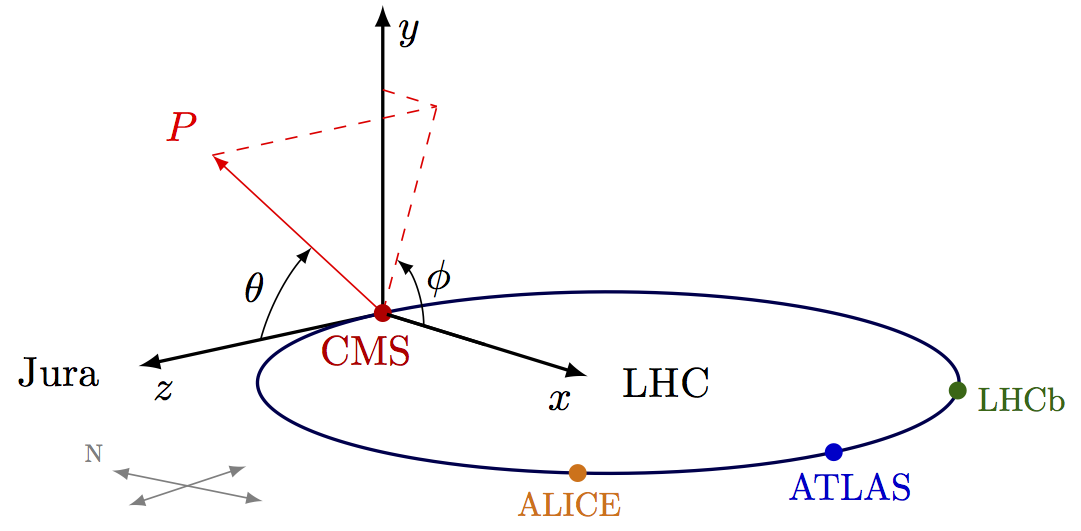
\includegraphics[width=0.8\textwidth]{Images/coordinatechart.png}
	\captionof{figure}{Coordinate system employed by the CMS experiment (retrieved from~\parencite{cmsplots}).}\label{fig_coordinates}
\end{center}

The event rate $R$ for a physical process (e.g., $pp \to X$) is governed by the accelerator's luminosity $\mathcal{L}$ and the process cross section $\sigma$. Luminosity quantifies the performance of a collider to produce interactions, establishing the proportionality,
\begin{equation}
	\frac{d R}{d t} = \mathcal{L} \sigma,
\end{equation}
where $\sigma$ (typically measured in barns, $1\,\text{b} = 10^{-24}\,\text{cm}^2$) encodes the interaction probability. For LHC proton bunches colliding head-on with Gaussian transverse profiles, the instantaneous luminosity is~\parencite{Herr:941318,book:1123430}:
\begin{equation}
	\mathcal{L} = \frac{f N_{b}}{4\pi} \frac{N_{1} N_{2}}{\sigma_{x} \sigma_{y}}\label{eq_lumi}
\end{equation}
Here, $N_{1,2}$ are proton counts per bunch, $f$ is the bunch collision frequency, $N_{b}$ is the number of bunches, and $\sigma_{x,y}$ are transverse beam widths. 

Integrating $\mathcal{L}$ over time yields the total integrated luminosity $L$, linking directly to the observed event count $N$:
\begin{equation}
	L = \int \mathcal{L}\, dt \quad \Rightarrow \quad N = L \sigma.
\end{equation}
%At Run~II luminosities ($\mathcal{L} \approx 1.5 \times 10^{34}\,\text{cm}^{-2}\text{s}^{-1}$), a $1\,\text{pb}$ cross section produces $\sim\!15$ events per second. This framework underpins all LHC physics analyses, from Higgs measurements ($\sigma_{pp\to H} \sim 50\,\text{pb}$ at $13\,\text{TeV}$) to BSM searches for rare processes ($\sigma_{\text{BSM}} \ll 1\,\text{fb}$).
  
The Gaussian beam approximation in~\eqref{eq_lumi} ignores hourglass effects (beam divergence near interaction points) and dynamic $\sigma_{x,y}$ variations during fills. CMS mitigates these via real-time luminosity monitoring using pixel clusters~\parencite{Sirunyan2021}, with systematic uncertainties below $2\%$. High $\mathcal{L}$ also introduces pileup—multiple $pp$ interactions per bunch crossing—which complicates $\eta$/$\phi$ measurements but is corrected using vertex isolation algorithms.


The most important parameters of an accelerator are the following:
\begin{description}

	\item[Centre-of-mass energy]  $(\sqrt{s})$ The energy of the colliding particles in the centre-of-mass (CM) frame. Since the total momentum of the particles in the CM frame is zero, the CM energy is simply the square-root of the total 4-momentum:
	$$
	\begin{gathered}
		\sqrt{s}=\sqrt{P^{\mu} P_{\mu}}, \\
		P^{\mu}=\sum_{i} p_{i}^{\mu}.
	\end{gathered}
	$$
	The energy in the CM frame must be greater than the total mass of the particles being produced. Thus, the CM energy determines which particles can be studied in the accelerator.
\end{description}
\begin{center}
  		% CMS detector - left perspective
		\tdplotsetmaincoords{75}{50} % to reset previous setting
		\begin{tikzpicture}[scale=2.6,tdplot_main_coords,rotate around x=90]
			
			% VARIABLES
			\def\rvec{\L/2/cos(\thetavec)}
			\def\thetavec{18}
			\def\phivec{60}
			\def\L{3.3}    % detector length
			\def\R{0.75}   % detector cylinder radius
			\def\l{4.3}    % beam pipe length
			\def\r{0.04}   % beam pipe radius
			\def\rt{0.042} % beam pipe radius + line thickness
			\def\xmax{1}   % maximum x axis
			\def\ymax{1}   % maximum y axis
			\def\zmin{-\l/2-0.2} % minimum z axis
			\def\zmax{\l/2+0.3}  % maximum z axis
			\def\w{0.3}
			\coordinate (O) at (0,0,0);
			\coordinate (Z) at (0,0,\L/2);
			\tdplotsetcoord{O'}{0.022}{\thetavec}{\phivec} % slightly shifted origin
			\tdplotsetcoord{O''}{0.018}{90}{\phivec} % slightly shifted origin
			\tdplotsetcoord{P}{\rvec}{\thetavec}{\phivec}
			
			% CYLINDER behind
			\def\ang{19} % rotate lines to simulate cylinder
			\fill[top color=red!50!black!4,bottom color=red!60!black!2,rotate around z=\ang]
			(0,\R,\L/2) --++ (0,0,-\L) arc(90:270:\R) --++ (0,0,\L) arc(270:90:\R) -- cycle;
			\fill[detector surface] % transverse plane at z=L/2
			(0,0,\L/2) --++ (0,\R,0) arc(90:270:\R) -- cycle;
			\fill[detector surface] % transverse plane at z=-L/2
			(0,0,-\L/2) --++ (0,\R,0) arc(90:270:\R) -- cycle;
			\tdplotdrawarc[detector]{(0,0,\L/2)}{\R}{0}{360}{}{}
			\tdplotdrawarc[detector,thin]{(0,0,-\L/2)}{\R}{0}{360}{}{}
			%\draw[detector,canvas is yx plane at z=-\L/2] (0,0,0) circle(\R);
			\draw[detector,thin, dashed] % transverse plane at z=0
			(90-\ang:\R) arc (90-\ang:270:\R);
			\draw[detector] (0,0,-\L/2)++(90:\R) --++ (0,0,\L); % top horizontal
			\draw[detector] (0,0,-\L/2)++(-90:\R) --++ (0,0,\L); % bottom horizontal
			
			% BEAM PIPE
			\tdplotdrawarc[beam pipe]{(0,0,\l/2)}{\r}{0}{360}{}{}
			%\tdplotdrawarc[beam pipe]{(0,0,-\l/2)}{\r}{\ang-90}{90}{}{}
			%\draw[beam pipe] % cylindric beam pipe
			%  (0,\r,-\l/2) --++ (0,0,\l) arc(90:-90:\r)
			%  --++ (0,0,-\l) arc(-90:90:\r);
			\draw[beam pipe] % beam pipe, thinner in middle
			(0,\r,-\l/2) -- (0,\r,-0.2*\l) -- (90:0.5*\r)
			-- (0,\r,0.2*\l) -- (0,\r,0.5*\l) arc(90:-90:\r)
			-- (0,-\r,0.2*\l) -- (-90:0.5*\r) --
			(0,-\r,-0.2*\l) -- (0,-\r,-\l/2) arc(-90:90:\r);
			\draw[beam pipe] (0,0,\l/2) circle(\r);
			
			% AXES
			%\draw[thick,->] (0,0,0) -- (0,0,1) node[below right]{$z$}; % short
			\draw[axis,-] (0,0,\zmin) -- (0,0,0); % long
			\fill[CMScol] (O) circle(0.5pt) node[right=1,below=1] {IP};
			\draw[axis] (0,0,0.020) -- (0,0,\zmax) node[right=3,above=0.1]{$z$}; % long
			\draw[axis] (0,0.019,0) -- (0,\ymax,0) node[below left]{$y$};
			\draw[axis] (0.022,0,0) -- (\xmax,0,0) node[below=1,right=-2]{$x$};
			
			% LABELS
			\node[mydarkred,above] at (0,\ymax,0) {$\eta=0$};
			\node[mydarkred,above=0.6, left] at (0,\R,0.3*\L) {$\eta>0$};
			\node[mydarkred,above=0.7, right] at (0,\R,-0.2*\L) {$\eta<0$};
			\node[mydarkred,below=1,left] at (0,0,\zmax) {$\eta=\infty$};
			\node[mydarkred,above=1,right] at (0,0,\zmin) {$\eta=-\infty$};
			
			% VECTORS
			%\fill[radius=0.4,red] (P) circle;
			\draw[dashed,myred] (P)  -- (Pxy);
			\draw[dashed,myred] (Py) -- (Pxy);
			\draw[dashed,myred] (P) -- (Pz);
			
			
			\draw[->,miverde,line cap=round,draw opacity=0.9] (O') -- (P) node[anchor=-30] {\contour{white}{$\va*{p}$}};
			\draw[->,miverde,line cap=round] (O') -- (P) node[anchor=-30] {$\va*{p}$};
			
			\draw[->,azulF,line cap=round,draw opacity=0.9] (O') -- (Pxy) node[right, anchor=-100] {\contour{white}{$\va*{p}_T$}};
			% \draw[->,azulF,line cap=round] (O') -- (Pxy) node[right , anchor=-100] {$\va*{p}_T$};
			
			
			% CYLINDER front
			\draw[beam pipe,fill=none] (0,\r,-\l/2) arc(90:-90:\r);
			\fill[detector surface] % transverse plane at z=L/2
			(0,\rt,\L/2) --++ (0,\R-\rt,0) arc(90:-90:\R) --++ (0,\R-\rt,0) arc(-90:90:\rt);
			\fill[detector surface] % transverse plane at z=-L/2
			(0,\rt,-\L/2) --++ (0,\R-\rt,0) arc(90:-90:\R) --++ (0,\R-\rt,0) arc(-90:90:\rt);
			\tdplotdrawarc[detector]{(0,0,\L/2)}{\R}{-90}{90}{}{} % transverse plane at z=L/2
			\tdplotdrawarc[detector]{(0,0,-\L/2)}{\R}{-90}{90}{}{} % transverse plane at z=-L/2
			\draw[beam pipe,fill=none] (0,\r,\l/2) arc(90:-90:\r);
			\draw[detector,very thin, dashed] % transverse plane at z=0
			(90-\ang:\R) arc (90-\ang:-90:\R);
			
			% ANGLES
			\tdplotdrawarc[thick,red!57!black!3] % contour
			{(O)}{0.2}{4}{0.7*\phivec}{}{}

			% white to contour
			\tdplotdrawarc[draw=azulF, line width=0.6pt, draw opacity=0.9]{(O)}{0.2}{0}{\phivec}{above=2,right=0.75,anchor=-30,text=black}{\contour{white}{$\phi$}}
			\tdplotdrawarc[->, azulF]{(O)}{0.2}{0}{\phivec}{above=2,right=0.75,anchor=-30}{$\phi$}


			\tdplotdrawarc[->,rotate around z=\phivec-90,rotate around y=-90]
			{(O)}{0.88}{0}{\thetavec}{anchor=mid east}{$\theta$}
			\tdplotdrawarc[thick,red!58!black!4,rotate around z=\phivec-90,rotate around y=-90] % contour
			{(O)}{0.3}{88}{0.5*(90+\thetavec)}{}{}
			\tdplotdrawarc[-{>[flex'=1]},rotate around z=\phivec-90,rotate around y=-90,line cap=round]
			{(O)}{0.3}{90}{\thetavec}{above=4.5,right=0.5,anchor=mid east}{$\eta$}
			\draw[mydarkred] (0,0,\L/2) --++ (\R,0,0);
			\tdplotdrawarc[thick,red!60!black!6] % contour
			{(Z)}{0.2}{4}{0.7*\phivec}{}{}
			\tdplotdrawarc[draw=none,opacity=0.8]{(Z)}{0.2}{0}{\phivec}{above=2,right=0.7,anchor=-30}{\contour{red!60!black!6}{$\phi$}}
			\tdplotdrawarc[->]{(Z)}{0.2}{0}{\phivec}{above=2,right=0.7,anchor=-30}{$\phi$}
			
			% COMPASS - CMS-ATLAS axis has a ~12° declination (http://googlecompass.com)
			\begin{scope}[shift={(1.1*\R,-\R,0.2*\L)},rotate around y=12]
				\draw[<->,black!50] (-\w,0,0) -- (\w,0,0);
				\draw[<->,black!50] (0,0,-\w) -- (0,0,\w);
				\node[left,black!50,scale=0.6] at (-\w,0,0) {N};
				\node[below=3,left=-2,green!20!black!50,scale=0.6] at (0,0,\w) {Jura};
				%\node[below=1,right,black!50,scale=0.6,align=center] at (\w,0,0) {center of\\the LHC};
				%\node[below=1,right,blue!30!black!50,scale=0.6] at (\w,0,0) {ATLAS};
			\end{scope}
			\draw[->,thick,orange!30!black] (1.4*\w,-\R,-0.1*\L) --++ (2*\w,0,0)
			node[right,scale=0.8,align=center] {center of\\[-1pt]the LHC};
			
		\end{tikzpicture}
  \captionof{figure}{Detailed reparametrization of the coordinate system employed by the CMS experiment (retrieved from~\parencite{cmsplots})}\label{fig_cms_coor}
\end{center}
The following variables are related to the particles being produced rather than the accelerator.
\begin{description}
	\item[Decay width] ( $\Gamma)$ The decay rate is the probability that a given particle will decay per unit time. Since a particle can have multiple decay modes, the total decay rate is the sum of the decay rates for each mode~\parencite{book:1123430}. The relative frequency of a decay mode is the branching ratio, given by
	$$
	\mathrm{BR}(j)=\frac{\Gamma(j)}{\Gamma} .
	$$
	\item[Cross-section] $(\sigma)$ The cross-section is a measure of the probability that an interaction will occur from a collision. It is a quantum-mechanical analogue of the "effective size" of the particles involved in an interaction.

	\item[Pseudo-rapidity] $(\eta)$ Instead of using the polar angle, CMS measurements involve the pseudo-rapidity, defined by
	$$
	\eta=-\ln \left(\tan \frac{\theta}{2}\right)
	$$
	The main advantage of using the pseudo-rapidity is that distributions over it tend to be closer to a uniform distribution than those over the polar angle, see Fig.~\ref{fig_cms_coor}. Furthermore, the difference in pseudo-rapidity is invariant under Lorentz boosts along the beam direction~\parencite{book:1123430}.
	\item[Transverse Momentum] ($p_T$) Refers to the component of momentum which is perpendicular to the beam line. It is usually preferred over full momentum because momentum along the beamline may just be left over from the beam particles, while the transverse momentum is always associated with whatever physics happened at the vertex, see Fig.~\ref{fig_cms_coor}.
	\item[Missing transverse energy and momentum] $\left(E_{T}^{\text {miss }} \& p_{T}^{\text {miss }}\right)$ Missing energy and momentum refers to the energy and momentum that is not detected but is expected to be there as a consequence of energy conservation and momentum conservation. This momentum is often carried by particles that do not interact electromagnetically or strongly and are therefore difficult to detect~\parencite{book:1123430}. Missing energy and momentum provides an indirect measurement of undetectable particles in hadron colliders such as neutrinos. Missing momentum reconstructions focus on the transverse direction, where total momentum is expected to be zero.
\end{description}


\section{Detectors and Subsystems}

A typical collider experiment comprises several main detector subsystems that are used jointly to detect and measure the properties of particles produced in the collision. A \textit{schematic representation} of such a generic multipurpose detector is shown in Fig.~\ref{fig_detector}. The detector is typically composed of several concentric layers, each designed to measure different properties of the particles produced in the collisions. 

\begin{center}
	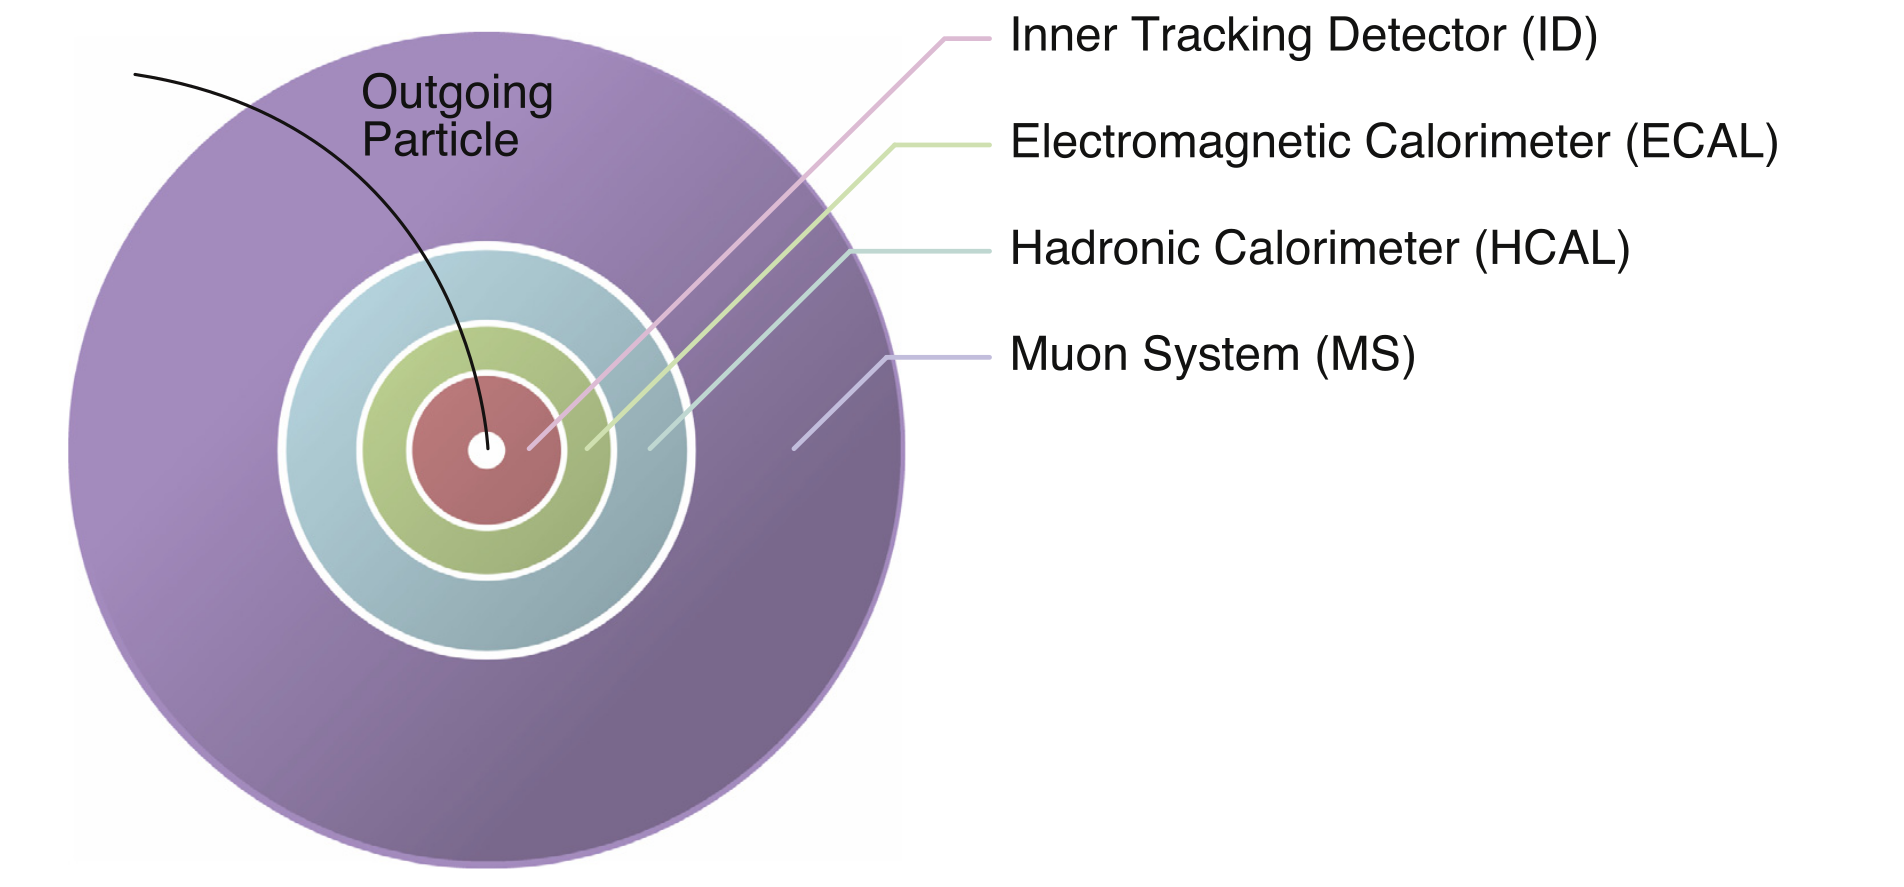
\includegraphics[width=0.98\textwidth]{Images/detector.png}
	\captionof{figure}{Schematic representation of a generic multipurpose detector (retrieved from~\parencite{cmsplots})}\label{fig_detector}
\end{center}

The innermost subsystem, called the inner detector (ID), is designed to detect electrically charged particles that are long-lived enough to traverse the ID. The most common such particles from the SM are two charged leptons (the electron $e$ and the muon $\mu$ ) and three hadrons (the pion $\pi$, kaon $K$, and proton $p$ ). Regions of ionization produced by such a particle in solid-state or gaseous detector sensors are detected as spatial hits that are fit into a trajectory, referred to as a track. The direction and curvature of the track in a magnetic field yield the particle's momentum vector and electric charge. In some detectors, the ID is enclosed in a Cherenkov-light detector used to measure the velocity of the tracked particles. Combined with the momentum measurement in the ID, this yields the particle mass with sufficient resolution to differentiate between pions, kaons, and protons in a relevant momentum range.

After passing through the tracker, particles produced in the collisions typically enter an electromagnetic calorimeter (ECAL), designed to measure the energies of photons, electrons and positrons. The energy measurement exploits the properties of electromagnetic shower production via photon radiation and $e^{+} e^{-}$ pair production, resulting from the interaction of energetic particles with the ECAL material.

Hadrons deposit energy via hadronic interactions with the detector material. Since this process involves large fluctuations and a variety of energy-deposition mechanisms, precise hadron-energy measurement is achievable only at high-energy colliders, where fluctuations are effectively averaged out. In particular, high-energy quarks and gluons hadronize into a collimated spray of hadrons known as a jet. Containing the jet requires use of a deep hadronic calorimeter (HCAL) beyond the ECAL. While a jet can be identified solely in the calorimeters, its energy is nowadays measured from a combination of the momenta of tracks in the ID and the signals integrated in the ECAL and HCAL.

Muons do not undergo hadronic interactions, and are heavy enough that they lose energy due to ionization at a low rate. Therefore, they lose only a few GeV while traversing a typical LHC-detector calorimeter. Using this property to identify them, a muon system (MS) is built outside the calorimeter. In high-energy collider detectors, the MS is usually immersed in a magnetic field in order to measure the momenta of muons. Tracks reconstructed in the MS are often combined with tracks in the ID to obtain a high-quality momentum measurement.

When studying final states that include long-lived, weakly interacting particles, such as neutrinos in the SM, an important reconstructed quantity is missing momentum. Using three-momentum conservation and the approximate hermeticity of the detector, it is possible to measure the momentum imbalance in the event and to infer the combined momentum of the invisible set of particles. Since the interacting partons in proton collisions generally carry different fractions of the momenta of the incoming hadrons and many of the particles produced fall outside of the acceptance of the sensitive detector, the summed momenta of measured final-state particles along the beam axis $z$ are not expected to cancel. Therefore, experiments at the LHC and Tevatron measure the missing transverse momentum, denoted $E_{\mathrm{T}}^{\text {miss }}$ or MET, where momentum balance is assumed only in the $x-y$ plane transverse to the beam direction.

Collider detectors are mostly designed and constructed for optimal detection of SM particles produced in the collision. However, they can also be used to search for new physics (NP) beyond the SM. In this case, the detector is used to search for signatures of NP, such as new particles or interactions that are not predicted by the SM. The detector subsystems are designed to be sensitive to a wide range of particles and interactions, allowing for the detection of a variety of NP signatures.

\subsection{Jets Reconstruction}

At the LHC, jets are reconstructed as proxies for the quarks and gluons produced in the hard scattering process. Due to color confinement, these partons cannot be observed directly, and instead hadronize into collimated sprays of particles. These sprays are clustered into jets using algorithms that group together the signals of their constituents in the detector.

The most widely used algorithm in ATLAS and CMS is the anti-$k_T$ clustering algorithm~\parencite{Cacciari:2008gp}, implemented in the \texttt{FastJet} package~\parencite{Cacciari:2011ma}. This algorithm groups particle candidates or calorimeter deposits into jets based on their proximity in the rapidity-azimuth $(y,\phi)$ plane, with a distance parameter $R$ typically set to values like 0.4 or 0.6. The resulting jets have a regular conical shape and are relatively insensitive to soft radiation and pileup.

Modern jet reconstruction exploits particle-flow (PF) algorithms, which combine information from all detector subsystems to reconstruct individual particles (charged hadrons, neutral hadrons, photons, electrons, and muons). The momenta of PF candidates are then used as input for jet clustering. This approach improves the resolution of jet energy and direction, especially at low transverse momentum.

After clustering, several levels of jet energy corrections (JEC) are applied to account for detector response, pileup, and underlying event contributions. These corrections are derived from simulation and in-situ calibrations using well-known processes like dijet balance or photon+jet events.

\subsection{$\tau$ Tagging at Multipurpose Detectors}

The tau lepton, being the heaviest charged lepton in the SM, decays promptly into either a lighter lepton (electron or muon) and neutrinos, or into hadrons and a tau neutrino. About 65\% of taus decay hadronically, producing narrow jets with a characteristic signature.

Hadronic tau decays ($\tau_{\text{had}}$) typically produce one or three charged hadrons (predominantly pions) and up to two neutral pions, which decay into photons. These decay products result in a collimated energy deposit in the calorimeters and a small number of associated tracks. Tau jets are thus narrower than QCD jets and have lower track multiplicity.

Tau identification algorithms at the LHC exploit these features by using multivariate techniques that combine:
\begin{itemize}
    \item the number of charged and neutral constituents,
    \item the collimation of energy deposits,
    \item isolation criteria based on the surrounding activity,
    \item the invariant mass of the visible decay products,
    \item and lifetime-related variables (e.g., impact parameter significance).
\end{itemize}

In CMS, the Hadron Plus Strips (HPS) algorithm reconstructs the decay mode and applies discriminants to distinguish taus from jets, electrons, and muons~\parencite{CMS:2022ydz}. ATLAS uses similar methods, with Boosted Decision Trees (BDTs) trained to separate taus from background~\parencite{ATLAS:2022fgo}.

Typical tau tagging efficiencies are around 60\% for hadronic taus, with misidentification rates of about 1\% for quark/gluon jets, depending on the working point.

\subsection{B Tagging at Multipurpose Detectors}

Jets originating from bottom quarks ($b$-jets) exhibit distinct features due to the relatively long lifetime ($\sim 1.5$ ps) and large mass ($\sim 4.2$ GeV) of the $b$ hadrons. These hadrons travel a few millimeters before decaying, often producing secondary vertices displaced from the primary interaction point.

$b$-tagging algorithms exploit this property by reconstructing tracks with large impact parameters and identifying displaced secondary vertices. Some algorithms also make use of the presence of soft leptons inside the jet from semileptonic $b$ decays.

Classical algorithms include:
\begin{itemize}
    \item \textbf{Track Counting:} based on the number of tracks with high impact parameter.
    \item \textbf{Jet Probability:} uses the probability that the jet’s tracks originate from the primary vertex.
    \item \textbf{Secondary Vertex:} reconstructs displaced vertices within the jet.
\end{itemize}

Modern approaches rely on machine learning techniques to combine multiple observables. CMS uses DeepCSV and DeepJet algorithms~\parencite{CMS:2017wtu}, based on deep neural networks. ATLAS employs algorithms like MV2 and DL1~\parencite{ATLAS:2019bwq}. These classifiers achieve improved performance in distinguishing $b$-jets from $c$-jets and light-flavor jets.

Typical $b$-tagging efficiencies range from 60\% to 80\%, depending on the working point, with light-jet misidentification rates of 1\% or lower. Calibrations are performed using data-driven methods in control samples enriched in $t\bar{t}$ or multijet events.

\subsection{The CMS Detector}
Particularly the CMS multi-purpose detector has a length of $21.6$ meters, with a diameter of $14.6$ meters and weights 12500 tonnes. The detector is composed of a set of different sub-detectors as seen in figure \ref{fig_cms}. The CMS detector has a cylindrical shape and it is divided into two main sections: barrel and endcaps. 

\begin{center}
	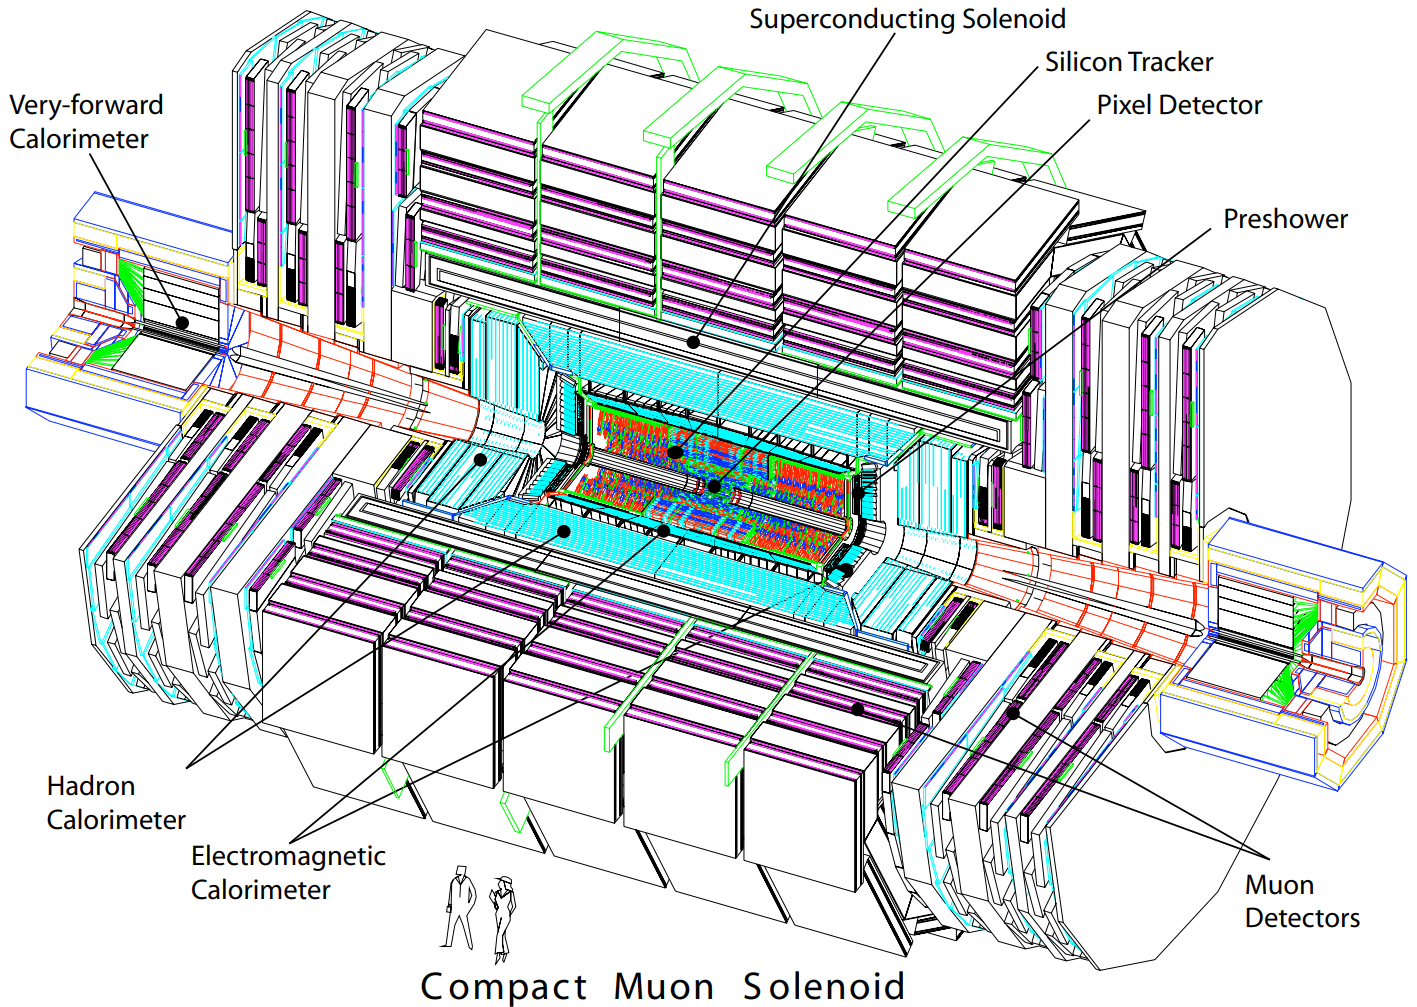
\includegraphics[width=0.98\textwidth]{Images/CMS.png}
	\captionof{figure}{Diagram of the CMS detector showing inner components (retrieved from~\parencite{Collaboration_2008})}\label{fig_cms}
\end{center}

The different sub-detectors are located concentrically in layers~\parencite{Collaboration_2008}. The inner most layer has a pixel detector made out of silicon, used for the reconstruction of primary and secondary vertices from electrically charged particles that decay promptly within this sub-detector volume. The pixel detector is followed by a sub-detector made of silicon strips, known as the tracker detector, used for the reconstruction of trajectories of electrically charged particles. Following the tracker detector, are found the electromagnetic (ECAL) and hadron (HCAL) calorimeters, used to measure both energy and direction of the particles undergoing electromagnetic and strong interactions, respectively. The ECAL detector is a modular device composed of lead-tugsten crystals, highly efficient to produce electromagnetic showers after interacting with charged particles. The emerging photons from the showers are measured using photo-diodes, that collect the light produced from the signal and convert it into an electric signal. This signal is then used by software tools to detect the energy and direction of the corresponding particles~\parencite{Collaboration_2008}. The ECAL is made of non magnetic materials such as copper and steel, which are characterized by heavy nuclei favoring strong interactions. Following a similar functioning as ECAL, hadronic particles enter the calorimeter, interact with the non-magnetic layers producing hadronic showers. These showers are then detected by plastic scintillators and their signals are transformed into electric pulses. These signals are then analyzed to estimate the energy and direction of the original particles~\parencite{Collaboration_2008}.

The next layer of the detector consists of a superconducting solenoid, which surrounds the previous sub-detectors. This solenoid is made of a niobum-titanium alloy that is refrigerated to $2 \mathrm{~K}$ by using liquid helium, producing a uniform magnetic field of $3.8 \mathrm{~T}$ inside the barrel~\parencite{Collaboration_2008}. This magnetic field is used to measure the momentum of electrically charged particles as it induces curvatures in their trajectories.

Finally, the last set sub-detectors conform the muon detector system. This system is made of three different detector technologies, that allow to reconstruct the trajectory of the muons with a fast trigger response, and are alternated with iron returning yokes of steel to enclose the magnetic field produced by the solenoid. The trigger is a date-filtering system composed of hardware and software algorithms, designed to collect interesting events from the proton-proton collisions. The muon detectors have a total of 1400 chambers distributed in 250 drift tubes, 540 cathode strip chambers that track the position of a muon and provide a trigger, as well as 610 resistive plate chambers that give a redundant trigger, which quickly decide over the event storage~\parencite{Collaboration_2008}.

% To do: ADD related with aceptance and efficiency in the barrel and endcaps.

Due to its cylindrical geometry, the CMS detector is divided into a central barrel region and two forward endcaps, which define the detector acceptance in terms of the pseudorapidity. The barrel region provides coverage for $|\eta| \lesssim 1.5$, while the endcap regions extend the acceptance up to $1.5\lesssim|\eta| \lesssim 2.5$ for most subsystems~\parencite{Collaboration_2008}. 

This geometrical segmentation impacts the overall detection efficiency. For example, the pixel and silicon strip trackers are more efficient in the barrel, where multiple tracking layers are crossed perpendicularly by particles. In the endcaps, particles cross detector layers at shallow angles, leading to reduced hit multiplicity and, consequently, lower tracking efficiency and resolution. Similar considerations apply to the ECAL and HCAL subsystems, where the granularity and material budget have been optimized to compensate for the non-uniform geometry, maintaining energy resolution across $\eta$.

Muon identification and momentum reconstruction also exhibit regional differences. The drift tubes (DTs), which offer high spatial resolution, are only installed in the barrel, while cathode strip chambers (CSCs) and resistive plate chambers (RPCs) cover the endcap regions. The combination of technologies ensures redundancy and robust triggering throughout the full detector acceptance. However, due to the higher background levels and increased radiation in the endcaps, the performance of muon reconstruction tends to be better in the barrel. For muons (electrons), the assumed identification efficiency is 95\% (85\%), with a 0.3\% (0.6\%) mis-identification rate~\parencite{CMS-PAS-FTR-13-014,CMS_MUON_17001,CMS_EGM_17001}.

Following reference~\parencite{CMS_BTV2016}, we use a flat identification efficiency for $\bq$ jets of 70\% across the entire $\pt$ spectrum with misidentification rate of 1\%. These values correspond with the  ``medium working point'' of the CMS algorithm to identify $\bq$ jets, known as DeepCSV. We also explored the ``Loose'' (``Tight'') working point using an efficiency of 85\% (45\%) and mis-identification rate of 10\% (0.1\%). 

For the performance of $\tau_{\textrm{h}}$ identification in DELPHES, we consider the latest technique described in~\parencite{CMS_DeepTau}, which is based on a deep neural network (i.e. DeepTau) that combines variables related to isolation and $\tau$-lepton lifetime as input to identify different $\tau_{\textrm{h}}$ decay modes. Following~\parencite{CMS_DeepTau}, we consider three possible DeepTau ``working points'': (i) the ``Medium'' working point of the algorithm, which gives a 70\% $\tau_{\textrm{h}}$-tagging efficiency and 0.5\% light-quark and gluon jet mis-identification rate; (ii) the ``Tight'' working point, which gives a 60\% $\tau_{\textrm{h}}$-tagging efficiency and 0.2\% light-quark and gluon jet mis-identification rate; and (iii) the ``VTight'' working point, which gives a 50\% $\tau_{\textrm{h}}$-tagging efficiency and 0.1\% light-quark and gluon jet mis-identification rate. Similar to the choice of $\textrm{b}$-tagging working point, the choice of $\tau_{\textrm{h}}$-tagging working point is determined through an optimization process which maximizes discovery reach. The ``Medium'' working point was ultimately shown to provide the best sensitivity and therefore chosen for this study. 

\section{Phenomenological Pipeline}
For the study of hypothetical signals for these new models and their feasibility of observation in experiments such as the LHC, one of the most widely used methods is the generation of events in colliders via Monte Carlo computational simulations. Monte Carlo simulation (MC) are used to predict what we expect to see under certain conditions:

\begin{itemize}
	\item To perform calculations in an automated way, such as, cross sections and disintegration widths.
	\item To perform studies before having the data.
	\item To compute event selection efficiency / acceptance.
	\item To predict the amount of background events.
	\item To distinguish different signals.
\end{itemize}

Today, there is a wide set of independent and modular tools that simulate the different experimental stages and that allow us to calibrate and contrast with relative ease the simulated results with the experimental ones. For pp collision simulations, the use of MadGraph5\_aMC@NLO (MadGraph)~\parencite{Alwall_2014} framework is widespread.

MadGraph is a modular working environment, that is, simulation occurs in several stages. First MadGraph receives the information with the Feynman rules of a specific model in a format known as Universal Feynman Output (UFO) (which is generated from the Lagrangian in Wolfram Mathematica with the use of the FeynRules library~\parencite{ALLOUL20142250}), along with a parameter card with the numerical values of the free parameters of the Lagrangian. 

With this information MadGraph creates a directory with all the diagrams and amplitudes of a given process (Output folder). Then a subroutine known as MadEvent is run that generates \textit{hard scatter events} and creates a known output in LHE format with the information of the four vectors of each particle of the final state. Normally, to optimize the generation with MadEvent, we can modify the so-called run\_card such that the output partons are in a state to be subsequently reconstructed in the detector. If we generate events whose partons will be ignored by the detector we are wasting computational power. 

Then, we can take the information from the LHE output to simulate the parton shower and the hadronization of the final state. This process is typically done with Pythia8 (Pythia)~\parencite{2203.11601}, which is possibly the most complete MC generator to simulate the parton shower and the hadronization. Here, we have the advantage that it is implemented to run automatically within MadGraph. 

Pythia output is in HepMC2 format. With this information we run a software, DELPHES~\parencite{de_Favereau_2014}, that performs a fast simulation of the detector response to interactions with particles. The output of DELPHES is in ROOT format ready for a data analysis in ROOT framework. From this point, the analysis is similar to that done in each of the experiments using the data delivered by the detector, although with an extra processing layer such as tagging processes of some particle candidates, such as light jets, b-jets, and hadronic taus.

\section{Measurement of the Power of an Analysis}
\label{sec:power_analysis}

The statistical power of an analysis quantifies its sensitivity to discriminate between signal and background processes. For binned data following Poisson statistics, we define the power $\kappa$ as:

\begin{equation}
\kappa = \frac{\sum_i s_i w_i}{\sqrt{\sum_i \left(s_i + b_i\right) w_i^2}},
\label{eq:kappa_definition}
\end{equation}

where:
\begin{itemize}
    \item $s_i$ and $b_i$ are the expected signal and background events in bin $i$
    \item $w_i$ is the optimal weight for bin $i$, given by:
    \begin{equation}
        w_i = \ln\left(1 + \frac{s_i}{b_i}\right)
        \label{eq:optimal_weights}
    \end{equation}
\end{itemize}

\subsection*{Special Case: Single Bin Analysis}
For a single bin with strong signal ($s \gg b$), Eq.~\ref{eq:kappa_definition} reduces to the Poisson significance:

\begin{equation}
\kappa \approx \frac{s}{\sqrt{s + b}},
\label{eq:single_bin_kappa}
\end{equation}

\subsection*{Incorporating Systematic Uncertainties}
The power calculation can be extended to include systematic uncertainties by modifying the denominator:

\begin{equation}
\kappa_{\text{sys}} = \frac{\sum_i s_i w_i}{\sqrt{\sum_i \left[(s_i + b_i) + \sigma^2_{\text{sys,signal},i} + \sigma^2_{\text{sys,bkg},i}\right] w_i^2}},
\label{eq:kappa_with_systematics}
\end{equation}

where $\sigma_{\text{sys}}$ terms represent the systematic uncertainties on signal and background predictions.